\newpage
\section{Decision Trees}
%\begin{figure}[H]
%  \centering
%  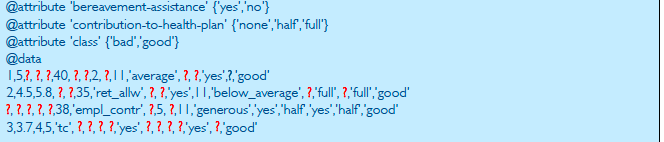
\includegraphics[width=.5\linewidth]{arffmissing}
%\end{figure}
\textbf{Decision Tree's} is an algorithm that has:
\begin{itemize}
\item \textbf{Internal Nodes}: which perform \textbf{tests} on \textbf{attributes}
\item \textbf{Branches}: that represent \textbf{outcomes} of the test
\item \textbf{Leaf Nodes}: represents a \textbf{class label} (or class label distribution)
\end{itemize}
At each node of the DT one attribute is chosen to \textbf{split} training samples into \textbf{distinct classes} as much as possible. After the model is computed , a new case is identified by following a \textbf{matching path} to a \textbf{leaf node}.

\subsection{Computing Decision Trees}
\begin{itemize}
\item \textbf{Top-down construction}\\
All training samples are at the root, then recursively partitioned by choosing one attribute at a time.
\item \textbf{Bottom-up Pruning}\\
Remove sub-trees or branches, in a bottom up manner to \textbf{improve} the estimated accuracy on new cases.
\end{itemize}
Decision Trees should separate classes in a \textbf{pure} way , that means that the separated areas contain mainly examples of one class. On this basis , DT implement a \textbf{purity} or \textbf{impurity} measure :
\begin{itemize}
\item ID3 $\rightarrow$ \textbf{information gain}
\item C4.5 $\rightarrow$ \textbf{information gain ratio}
\item CART $\rightarrow$ \textbf{gini index}
\end{itemize}


\subsubsection{Information Gain - ID3}
Information gain increases with the \textbf{average purity} of the subsets that an attribute produces . The \textbf{splitting strategy} chooses the attribute that results in the \textbf{largest information gain}.\\
Information is computed in \textbf{bits} : given a probability distribution the info required to predict an event is the \textbf{distribution's entropy} (which gives the information required in bits).
 $$ entropy(p_1,...,p_n) = -p_1logp_1 - p_2logp_2...-p_nlogp_n$$
So for each attribute the DT applies the \textbf{entropy measure} :
\begin{itemize}
\item outlook = sunny $\rightarrow entropy(\frac{2}{5},\frac{3}{5}) = .971$ 
\item outlook = overcast $\rightarrow entropy(\frac{5}{5},\frac{0}{5}) = .000$
\item outlook = rainy $\rightarrow entropy(\frac{3}{5},\frac{2}{5}) = .971$
\item $info([2,3],[4,0],[3,2]) \rightarrow \frac{5}{14} \cdot 0.971 + \frac{4}{14} \cdot 0 + \frac{5}{14} \cdot 0.971$
\end{itemize}
After computing the information , the \textbf{gain of information} (before and after split) must be computed : 
$$ gain(A) = info(D) - info_A(D)$$
where 
$$ info(D) = -p_1logp_1 - ... -p_nlogp_n$$
$$ info_A(D) = \frac{|D_1|}{D}info(D_1) + ...+  \frac{|D_n|}{|D|}info(D_n)$$
In our example :
\begin{itemize}
\item  gain(outlook) = $info([9,5])-info([2,3],[4,0],[3,2]) = .940 - .693 = 0.247$
\end{itemize}
The higher the gain, the better! The final tree looks like this:
\begin{figure}[H]
  \centering
  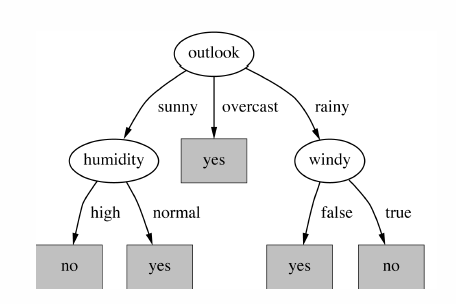
\includegraphics[width=.5\linewidth]{DTfinal}
\end{figure}
Splitting \textbf{stops}:
\begin{itemize}
\item All samples given a node belong to the same class
\item No further attributes available $\rightarrow$ majority voting
\item No samples left
\item No gain in splitting
\end{itemize}
 Using decision trees $100 \% $ accuracy can be achieved but it is \textbf{not} a desirable thing to have most of the time. For example an \textbf{ID} attribute, where each sample has a distinct value , will surely be picked by the algorithm as it results in the highest gain. But an ID will never be a good prediction indicator so will lead to \textbf{overfitting}.\\
 This is why Information gain is \textbf{biased} towards choosing attributes with a \textbf{large number of values}.
 
\subsubsection{Information Gain Ration - C4.5}
Modification of the Information Gain that \textbf{reduces bias towards highly-branched} attributes. Information gain should be:
\begin{itemize}
\item \textbf{Large} $\rightarrow$ data \textbf{evenly spread}
\item \textbf{Small} $\rightarrow$ data belong to \textbf{one branch}
\end{itemize}  
Information gain ratio takes \textbf{number} and \textbf{size} into account when choosing an attribute. The \textbf{intrinsic information } computes the entropy of distribution of instances into branches:
$$ IntrinsicInfo(S,A) = - \sum \frac{|S_i|}{|S|}log \frac{|S_i|}{S}$$
$$ GainRatio(S,A) =  \frac{Gain(S,A)}{IntrinsicInfo(S,A)}$$
So for example for an attribute like ID :
\begin{itemize}
\item Intrinsic Information $\rightarrow info([1,1,....,1])=14 \cdot (-\frac{1}{14} \cdot log \frac{1}{14})= 3.807 $
\item GainRatio(ID-Code) = $\frac{.940}{3.807}= 0.246$
\end{itemize}
C4.5 works also with \textbf{numerical attributes} :
\begin{enumerate}
\item sort all values and their class labels 
\item check \textbf{all cutting points} and choose the one with the best information gain
\end{enumerate}
Sorting instances by value takes $O(nlogn)$  but has to be done \textbf{once} since the ordering for children can be \textbf{derived} from the parents with derivation time $O(n)$ which requires to \textbf{store indices} for each numeric attribute.\\
Another feature of numeric attributes is that they can be used more than ones in different part of the tree. This can lead to very complex trees and is often a problem. Solutions:
\begin{itemize}
\item \textbf{Pre-discretize} numeric attributes
\item Use \textbf{multi-way splits} instead of binary splits.
\end{itemize}

\subsubsection{Gini Index - CART}
The Gini Index ,for a dataset T contains examples from n classes, is defined as 
$$ gini(T) = 1 - \sum \limits_{j=1}^{n}p^2_j$$
Where $p_j$ is the \textbf{relative frequency} of class j in T. The index is \textbf{minimized} if the classes in T are \textbf{skewed}.
\begin{figure}[H]
  \centering
  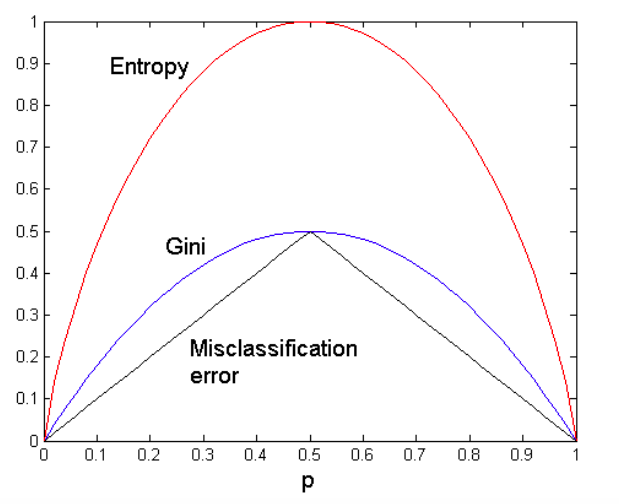
\includegraphics[width=.5\linewidth]{gini}
\end{figure}
Gini and entropy measure the same thing but have different shapes in relation to the frequency of a class.\\
If the dataset is split into two \textbf{subsets} by attribute A:
$$ gini_A(D) = \frac{|D_1|}{|D|} gini(D_1) + \frac{|D_2|}{|D|}gini(D_2)$$
With a reduction of \textbf{impurity}: 
$$ \Delta gini(A) = gini(D) - gini_A(D)$$
The attribute that provides the \textbf{smallest} Gini splitting D over A (or the \textbf{largest reduction in impurity} ) is chosen to split the node. This requires to enumerate all the possible splitting points for each attribute.
Example over the \texttt{Outlook} attribute :
\begin{itemize}
\item 9 tuples labeled yes , 5 labeled no :
$$ gini(D) = 1- \left( \frac{9}{14} \right)^2 - \left( \frac{5}{14} \right)^2 = 0.459$$
\item The attribute has \textbf{three} possible values so evaluate all possible partitions:
\begin{itemize}
\item (overcast,rainy) , (sunny)
$$ Gini(D_{o,r}, D_s)= \frac{9}{14}Gini(D_{o,r})+\frac{5}{14}Gini(D_s)$$
$$ = \frac{9}{14}Gini([7,2]) + \frac{5}{14}Gini([2,3]) =0.394$$
\item (rain,sunny) , (overcast)
$$ Gini(D_{r,s}, D_o)= \frac{10}{14}Gini(D_{r,s})+\frac{4}{14}Gini(D_o)$$
$$ = \frac{10}{14}Gini([5,5]) + \frac{4}{14}Gini([4,0]) =0.357$$
\item (overcast,sunny) , (rainy)
$$ Gini(D_{o,s}, D_r)= \frac{6}{2}Gini(D_{s,o})+\frac{3}{2}Gini(D_r)$$
$$ = \frac{6}{3}Gini([6,3]) + \frac{3}{2}Gini([3,2]) =0.457$$
\end{itemize}

\item The best partition is (rainy,sunny) , (overcast) with a gain of 
$$ Gini(D) - Gini(D_{r,s},D_o) =0.459 - 0.357 = .102 $$
\end{itemize}

\subsection{Overfitting and generalization}
A decision tree with too many branches may reflect \textbf{anomalies} or \textbf{outliers} : results in poor accuracy for unseen examples.
Solutions :
\begin{itemize}
\item Pre-pruning
\item Post-pruning
\end{itemize}

\subsubsection{Pre-pruning}
Pre-pruning bases its pruning technique on \textbf{statistical significance tests} : only statistical significant attributes were allowed to be selected by information gain procedure. The tree stops growing when there is no statistical significant \textbf{association} between any attribute and the class at a particular node.\\
The most popular test is the \textbf{Chi-Squared test} already used in the ID3 algorithm.

\subsubsection{Post-pruning}
Removes branches from \textbf{full-grown} trees applying :
\begin{itemize}
\item \textbf{Subtree raising}
\item \textbf{Subtree replacement}\\
Works bottom-up: it considers replacing a tree if and only if all its subtrees have been considered. This is done using again statistical tests.
\end{itemize} 
Using a strategy : 
\begin{itemize}
\item \textbf{Error estimation}\\
A branch/tree is pruned only if it reduces the \textbf{estimated error}. Error on training data is \textbf{not} a useful measure : keep an \textbf{hold-out set} for pruning (\textbf{reduced error pruning}).\\
C4.5 derives a \textbf{confidence interval} on the training data and uses a heuristic limit for pruning (Standard Bernoulli based method):
$$ e = \frac{ \left(f+ \frac{z^2}{2N} + z \sqrt{\frac{f}{N}-\frac{f^2}{N}+ \frac{z^2}{4N^2}} \right)}{ \left( 1+ \frac{z^2}{N}\right) }$$
If $c=25\% \rightarrow z= 0.69$ , f is the error on training data and N the number of instances covered by the leaf.
\item \textbf{Significance testing}
\item \textbf{MDL principle}
\end{itemize}

\subsection{Regression and model trees}
DT can also be used to perform regression working in the same way as classification trees : looking for the best split that minimizes the impurity measure and the standard deviation in the leaves is very small
$$ \text{impurity measure : SDR}= \sigma(D) - \sum \frac{|D_i|}{|D|}\sigma(D_i)$$
\begin{itemize}
\item D = original dataset
\item $D_i$= partitions
\item $\sigma$= standard deviation of the target attribute in the set.
\end{itemize}
Prediction is computed as the \textbf{average} of numerical target variables in the subspace ( \textbf{regression trees}) or leaf nodes contain linear models to predict the target value (\textbf{ model trees})

\subsubsection{Decision Stumps}
Decision stumps are \textbf{one level decision trees} . They are very simple and also the main building block for \textbf{boosting methods}.
\begin{itemize}
\item \textbf{Categorical values}\\
One branch for each attribute, one branch for one value and one for the others; missing values a special value
\item \textbf{Numerical values}\\
Two leaves defined by a threshold value selected based on some criterion ; multiple splits
\end{itemize}